\documentclass[usepdftitle=false,hyperref={pdfpagelabels=false}]{beamer}
\usepackage{../templates/myStyle}

\begin{document}
\title{\titleText}
\subtitle{String interning, Assertions, Einfach verkettete Listen}
\author{\tutor}
\date{3. Dezember 2012}
\subject{Programmieren}

\frame{\titlepage}

\frame{
    \frametitle{Inhaltsverzeichnis}
    \setcounter{tocdepth}{1}
    \tableofcontents
    \setcounter{tocdepth}{2}
}

\section{Einleitung}
\subsection{Quiz}
\begin{frame}{Quiz}
    \inputminted[linenos=true, numbersep=5pt, tabsize=4, fontsize=\tiny]{java}{QuizString.java}
    \begin{itemize}
        \item Gibt es einen Compiler-Fehler? \xmark
        \item Gibt es einen Laufzeit-Fehler? \xmark
        \item Gibt es eine Ausgabe? \cmark{} Welche Ausgabe gibt es?
    \end{itemize}
\end{frame}

\begin{frame}{Quiz: Antwort}
    \inputminted[linenos=true, numbersep=5pt, tabsize=4, fontsize=\tiny]{java}{QuizString.java}
    \begin{itemize}
        \item string1 und string2 sind verschiedene Objekte.
        \item string3 und string4 sind das selbe Objekt.
    \end{itemize}
\end{frame}

\begin{frame}{Quiz: Erklärung}
    \begin{itemize}[<+->]
        \item Erstellt man einen String mit \myCode{String abc = new String("Hallo");}
              wird ein neues Objekt angelegt
        \item Erstellt man einen String mit \myCode{String abc = "Hallo";}
              macht Java "`String interning"'
    \end{itemize}
    \pause[\thebeamerpauses]
    \begin{alertblock}{Achtung}
        Trotzdem mit \myCode{abc.equals(def);} vergleichen! Nur so
        ist garantiert, dass ihr auf Gleichheit (und nicht nur auf
        "`Selbstheit"' vergleicht).
    \end{alertblock}
\end{frame}

\section{Assertions}
\subsection{Allgemeines}
\begin{frame}{Assertions}
    \begin{itemize}[<+->]
        \item Problem: Es tritt ein falsches Ergebnis auf, es ist
              aber nicht klar warum.
        \item Lösung: Man macht Zusicherungen (engl. assertions)
        \item Man überlegt sich also, welche Variablen an
              krischen Stellen welche Werte oder Beziehungen
              zueinander haben sollen
    \end{itemize}
    \pause[\thebeamerpauses]
    \begin{alertblock}{Wichtig: Assertions sind keine Exceptions!}
        \begin{tabular}{l|l}
            \textbf{Assertion}                  & \textbf{Exception}\\
            \hline
            muss man aktivieren                 & wird immer ausgeführt\\
            dient zum Entdecken von Fehlern     & dient zum behandeln von Fehlern\\
            z.B. (a < b), (a !=0), \dots        & z.B. \href{http://docs.oracle.com/javase/7/docs/api/java/io/IOException.html}{IOException}\\
        \end{tabular}
    \end{alertblock}
\end{frame}

\begin{frame}{Beispiel}
    \inputminted[linenos=false, tabsize=4, fontsize=\small]{java}{singleLines.java}
\end{frame}

\begin{frame}{Assertions aktivieren}
    In Eclipse:
    \begin{itemize}
        \item \menu{Window > Preferences > Java > Installed JREs > Edit...}
        \item Default VM Arguments: "`-enableassertions"' hinzufügen
    \end{itemize}
\end{frame}

\begin{frame}{Weitere Materialien}
    \begin{itemize}
        \item docs.oracle.com: \href{http://docs.oracle.com/javase/1.4.2/docs/guide/lang/assert.html}{Programming With Assertions}
        \item galileo openbook: \href{http://openbook.galileodesign.de/javainsel5/javainsel07_005.htm}{Java ist auch eine Insel}
        \item Java Blog Buch: \href{http://www.java-blog-buch.de/0609-assertions/}{06.09 Assertions}
    \end{itemize}
\end{frame}

\section{Einfach verkettete Listen}
\subsection{Allgemeines}
\begin{frame}{Einfach verkettete Listen}
    \begin{block}{Szenario}
      \begin{itemize}[<+->]
        \item Ihr wollt euch Druckaufträge speichern
        \item Funktioniert mit Array
        \item Problem:
          \begin{itemize}
            \item Ihr belegt immer konstant viel Speicher
            \item Eventuell braucht ihr mehr, eventuell weniger Speicher
          \end{itemize}
        \item Lösung: Verkettete Listen
      \end{itemize}
    \end{block}
\end{frame}

\begin{frame}{Idee}
    \begin{itemize}[<+->]
        \item Man speichert sich nur einen Zeiger
        \item Dieser Zeiger zeigt auf "`Knoten"'
        \item Jeder Knoten hat wieder einen Zeiger
        \item Jeder Knoten kann wieder auf einen Knoten zeigen
    \end{itemize}
    \only<\thebeamerpauses>{
        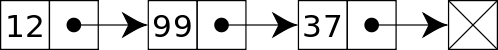
\includegraphics[width=\linewidth]{Singly-linked-list.png}
    }
\end{frame}

\framedgraphic{Weiteres Beispiel}{Listenbeispiel.jpg}

\begin{frame}{Was wollen wir?}
    \begin{itemize}[<+->]
        \item Elemente hinzufügen
        \item Elemente löschen
        \item Elemente finden
    \end{itemize}

    \pause[\thebeamerpauses]
    \begin{alertblock}{Wichtig}
        Zwischenergebnisse ausgeben
    \end{alertblock}
\end{frame}

\begin{frame}{Wie sieht das aus?}
    \inputminted[linenos=false, numbersep=5pt, tabsize=4, fontsize=\tiny, label=Main.java, frame=lines]{java}{Main.java}
\end{frame}

\begin{frame}{Welche Klassen brauchen wir?}
  \only<2>{
    \includegraphics[width=0.7\textheight]{ObjectDiagram.pdf}
  }
\end{frame}

\begin{frame}{Generics}
  \begin{block}{Hinweis}
    \begin{itemize}[<+->]
        \item Noch erstellt ihr eine Liste für genau einen Datentyp
        \item Eigentlich macht der Code immer das gleiche, ist also
              vom Datentypen unabhängig
        \item Das löst man später mit "`Generics"'
    \end{itemize}
  \end{block}

  \pause[\thebeamerpauses]
  \begin{block}{Hinweis 2}
    Oder - z.B. bei den Abschlussaufgaben - man verwendet einfach Datentypen
    aus \href{http://docs.oracle.com/javase/7/docs/api/java/util/package-summary.html}{java.util}:
    \begin{itemize}[<+->]
        \item \href{http://docs.oracle.com/javase/7/docs/api/java/util/LinkedList.html}{LinkedList}
        \item \href{http://docs.oracle.com/javase/7/docs/api/java/util/HashMap.html}{HashMap} /
              \href{http://docs.oracle.com/javase/7/docs/api/java/util/TreeMap.html}{TreeMap}
        \item \href{http://docs.oracle.com/javase/7/docs/api/java/util/HashSet.html}{HashSet} /
              \href{http://docs.oracle.com/javase/7/docs/api/java/util/TreeSet.html}{TreeSet}
    \end{itemize}
  \end{block}
\end{frame}

\subsection{Der Knoten}
\begin{frame}{Teil 1: Der Knoten}
    \begin{block}{Teil 1}
        Erstelle die Klasse Node
    \end{block}
    \includegraphics[width=0.7\textheight]{ObjectDiagram-list-node}
\end{frame}

\begin{frame}{Teil 1: Der Knoten}
    \inputminted[linenos=true, numbersep=5pt, tabsize=4, fontsize=\small, label=Node.java, frame=lines]{java}{Node.java}
\end{frame}

\subsection{Die Liste}
\begin{frame}{Teil 2.1: Die Struktur der Liste}
    \begin{block}{Teil 2.1}
        Erstelle die Klasse SinglyLinkedList (noch ohne Funktionalität)
    \end{block}
    \includegraphics[width=0.7\textheight]{ObjectDiagram-list-node}
\end{frame}

\begin{frame}{Teil 2.1: Die Struktur der Liste}
    \inputminted[linenos=true, numbersep=5pt, tabsize=4, fontsize=\tiny, label=SinglyLinkedList-structure.java]{java}{SinglyLinkedList-structure.java}
\end{frame}

\begin{frame}{Teil 2.2: printList()}
    \begin{block}{Teil 2.2}
        Erstelle die Methode "`printList"'
    \end{block}
    \includegraphics[width=0.7\textheight]{ObjectDiagram-list-node}
\end{frame}

\begin{frame}{Teil 2.2: printList()}
    \inputminted[linenos=true, numbersep=5pt, tabsize=4, fontsize=\tiny, firstnumber=60, firstline=60, lastline=69]{java}{SinglyLinkedList.java}
\end{frame}

\begin{frame}{Teil 2.3: Hilfsmethoden}
    \begin{block}{Teil 2.3}
        Erstelle die Methoden \myCode{boolean isEqual(Node node, int content)}
        und \myCode{Node findNode(int number)}
    \end{block}
    \includegraphics[width=0.7\textheight]{ObjectDiagram-list-node}
\end{frame}

\begin{frame}{Teil 2.3: Hilfsmethoden}
    \inputminted[linenos=true, numbersep=5pt, tabsize=4, fontsize=\tiny, firstnumber=5, firstline=5, lastline=21]{java}{SinglyLinkedList.java}
\end{frame}

\begin{frame}{Teil 2.4: append}
    \begin{block}{Teil 2.4}
        Erstelle die Methode \myCode{append}
    \end{block}
    \includegraphics[width=0.7\textheight]{ObjectDiagram-list-node}
\end{frame}

\begin{frame}{Teil 2.4: append}
    \inputminted[linenos=true, numbersep=5pt, tabsize=4, fontsize=\tiny, firstnumber=23, firstline=23, lastline=34]{java}{SinglyLinkedList.java}
\end{frame}

\begin{frame}{Teil 2.5: remove}
    \begin{block}{Teil 2.5}
        Erstelle die Methode \myCode{remove}
    \end{block}
    \includegraphics[width=0.7\textheight]{ObjectDiagram-list-node}
\end{frame}

\begin{frame}{Teil 2.5: remove}
    \inputminted[linenos=true, numbersep=5pt, tabsize=4, fontsize=\tiny, firstnumber=36, firstline=36, lastline=48]{java}{SinglyLinkedList.java}
\end{frame}

\begin{frame}{Teil 2.6: find}
    \begin{block}{Teil 2.6}
        Erstelle die Methode \myCode{find}
    \end{block}
    \includegraphics[width=0.7\textheight]{ObjectDiagram-list-node}
\end{frame}

\begin{frame}{Teil 2.6: find}
    \inputminted[linenos=true, numbersep=5pt, tabsize=4, fontsize=\tiny, firstnumber=50, firstline=50, lastline=58]{java}{SinglyLinkedList.java}
\end{frame}

\section{Abspann}
\subsection{Kommende Tutorien}
\begin{frame}{Kommende Tutorien}
  \begin{itemize}
    \item[7.] 03.12.2012: JUnit-Tests, \href{http://docs.oracle.com/javase/7/docs/api/java/lang/Object.html\#toString()}{toString}, Vererbung
    \item[6.] 10.12.2012: Generics?
    \item[5.] 17.12.2012: Video "`Library"' zeigen
    \item[-] 24.12.2012: Heiligabend - \href{http://www.fmc.uni-karlsruhe.de/faq/wann-sind-die-weihnachtsferien}{Kein Tutorium}
    \item[-] 31.12.2012: Silvester - Kein Tutorium
    \item[4.] 07.01.2013
    \item[3.] 14.01.2013
    \item[2.] 21.01.2013
    \item[1.] 28.01.2013: Abschlussprüfunsvorbereitung
    \item[0.] 04.02.2013: Abschlussprüfunsvorbereitung
    \item[-] 10.02.2013: Ende der Vorlesungszeit des WS 2012/2013 (\href{http://www.kit.edu/studieren/2873.php}{Quelle})
  \end{itemize}
\end{frame}

\framedgraphic{Vielen Dank für eure Aufmerksamkeit!}{../images/geekandpoke-development-cycle.jpg}

\end{document}
